%\documentclass[c]{beamer}  % [t], [c], или [b] --- вертикальное выравнивание на слайдах (верх, центр, низ)
%\documentclass[handout]{beamer} % Раздаточный материал (на слайдах всё сразу)


\documentclass[9pt,pdf]{beamer} % Соотношение сторон
\usepackage[labelfont=bf]{caption}
\usepackage{subfig} % for subfigures
\usepackage{bm}
%\usetheme{Bergen}
\usetheme{Berlin}
%\setbeamertemplate{footline}[frame number]
%\usetheme{Warsaw}

%\useoutertheme{тема}
%\useinnertheme{тема} 

\setbeamercolor{background canvas}{bg=white}
\useinnertheme[shadow]{rounded}

%%% Работа с русским языком
\usepackage{cmap}					% поиск в PDF
\usepackage{mathtext} 				% русские буквы в формулах
\usepackage[T2A]{fontenc}			% кодировка
\usepackage[utf8]{inputenc}			% кодировка исходного текста
\usepackage[english,russian]{babel}	% локализация и переносы
\usepackage{graphicx}
\usepackage{geometry}
\usepackage{lipsum}
%% Beamer по-русски
\newtheorem{rtheorem}{Теорема}
\newtheorem{rproof}{Доказательство}
\newtheorem{rexample}{Пример}

%%% Дополнительная работа с математикой
\usepackage{amsmath,amsfonts,amssymb,amsthm,mathtools} % AMS
\usepackage{icomma} % "Умная" запятая: $0,2$ --- число, $0, 2$ --- перечисление

%% Номера формул
%\mathtoolsset{showonlyrefs=true} % Показывать номера только у тех формул, на которые есть \eqref{} в тексте.
%\usepackage{leqno} % Нумерация формул слева
\usepackage{bm}
%% Свои команды
\DeclareMathOperator{\sgn}{\mathop{sgn}}
\newcommand{\myfigref}[2]{~\ref{#1}.\subref{#2}}% <---- a new macro for referring to a subfigure
% \myfigref{label: fig}{label: subfig}
\newcommand{\T}{^{\mathsf{T}}}
\DeclareMathOperator*{\argmax}{arg\,max}  % in your preamble
\DeclareMathOperator*{\argmin}{arg\,min}  % in your preamble 

%%% Работа с картинками
\usepackage{graphicx}  % Для вставки рисунков
\setlength\fboxsep{3pt} % Отступ рамки \fbox{} от рисунка
\setlength\fboxrule{1pt} % Толщина линий рамки \fbox{}
\usepackage{wrapfig} % Обтекание рисунков текстом

%%% Работа с таблицами
\usepackage{array,tabularx,tabulary,booktabs} % Дополнительная работа с таблицами
\usepackage{longtable}  % Длинные таблицы
\usepackage{multirow} % Слияние строк в таблице
\usepackage[labelfont=bf]{caption}
%%% Программирование
\usepackage{etoolbox} % логические операторы

%%% Другие пакеты
\usepackage{lastpage} % Узнать, сколько всего страниц в документе.
\usepackage{soul} % Модификаторы начертания
\usepackage{csquotes} % Еще инструменты для ссылок
%\usepackage[style=authoryear,maxcitenames=2,backend=biber,sorting=nty]{biblatex}
\usepackage{multicol} % Несколько колонок

%%% Картинки
\usepackage{tikz} % Работа с графикой
\usepackage{pgfplots}
\usepackage{pgfplotstable}

\title{Предсказание показания фМРТ по видео, показанному человеку}
\author{Дорин Даниил Дмитриевич}
\date{\today}
\institute[Московский физико-технический институт]{Московский физико-технический институт }

\setbeamercovered{transparent = 15}

\begin{document}

	\begin{frame}{}
		\maketitle
	\end{frame}
%%%%%%%%%%%%%%%%%%%%%%%%%%%%%%%%%%%%%%%%%%%%%%%%%%%%%%%%%%%%%%%%%%%%%%%%%%%%%%%%%%%%%%%%%%%%%%%%%%%%%%%%%%%%%%%%%%%%%%%%%%%%%%%%%%%%%%%%%%%%%%

%%%%%%%%%%%%%%%%%%%%%%%%%%%%%%%%%%%%%%%%%%%%%%%%%%%%%%%%%%%%%%%%%%%%%%%%%%%%%%%%%%%%%%%%%%%%%%%%%%%%%%%%%%%%%%%%%%%%%%%%%%%%%%%%%%%%%%%%%%%%%%
\begin{frame}{Цель работы}
    \begin{block}{Исследуется}
    Зависимость между показаниями датчиков фМРТ и видеорядом, просматриваемым человеком.
    \end{block}
    
    \begin{block}{Требуется}
    Предложить метод аппроксимации снимка фМРТ по видеоряду и нескольким дополнительным измерениям фМРТ того же испытуемого.
    \end{block}
    \begin{block}{Основные предположения}
    \begin{itemize}
        \item Наличие корреляции между снимками и изображениями из видеоряда.
        \item Реакция мозга, фиксируемая фМРТ, на информацию, поступающую от зрительных органов, происходит не мгновенно, а с некоторой задержкой $\Delta t$.
    \end{itemize}
    \end{block}
\end{frame}
%%%%%%%%%%%%%%%%%%%%%%%%%%%%%%%%%%%%%%%%%%%%%%%%%%%%%%%%%%%%%%%%%%%%%%%%%%%%%%%%%%%%%%%%%%%%%%%%%%%%%%%%%%%%%%%%%%%%%%%%%%%%%%%%%%%%%%%%%%%%%%

%%%%%%%%%%%%%%%%%%%%%%%%%%%%%%%%%%%%%%%%%%%%%%%%%%%%%%%%%%%%%%%%%%%%%%%%%%%%%%%%%%%%%%%%%%%%%%%%%%%%%%%%%%%%%%%%%%%%%%%%%%%%%%%%%%%%%%%%%%%%%%
\begin{frame}{Литература}
    \begin{block}{Набор данных}
    Julia Berezutskaya, Mariska~J. Vansteensel, Erik~J. Aarnoutse, Zachary~V. Freudenburg, Giovanni Piantoni, Mariana~P. Branco, and Nick~F. Ramsey.
    \newblock Open multimodal {iEEG}-{fMRI} dataset from naturalistic stimulation with a short audiovisual film.
    \newblock {\em Scientific Data}, 9(1), March 2022.
    \end{block}

    \begin{block}{Вспомогательные факты}
        Maxim Sharaev, Alexander Andreev, Alexey Artemov, Alexander Bernstein, Evgeny Burnaev, Ekaterina Kondratyeva, Svetlana Sushchinskaya, and Renat Akzhigitov.
        
        \newblock fmri: preprocessing, classification and pattern recognition.
        \newblock {\em Scientific Data}, 2018.
    \end{block}
\end{frame}
%%%%%%%%%%%%%%%%%%%%%%%%%%%%%%%%%%%%%%%%%%%%%%%%%%%%%%%%%%%%%%%%%%%%%%%%%%%%%%%%%%%%%%%%%%%%%%%%%%%%%%%%%%%%%%%%%%%%%%%%%%%%%%%%%%%%%%%%%%%%%%

%%%%%%%%%%%%%%%%%%%%%%%%%%%%%%%%%%%%%%%%%%%%%%%%%%%%%%%%%%%%%%%%%%%%%%%%%%%%%%%%%%%%%%%%%%%%%%%%%%%%%%%%%%%%%%%%%%%%%%%%%%%%%%%%%%%%%%%%%%%%%%
\begin{frame}{Постановка задачи}
Пусть $\bm{\Omega}$~--- видеоряд, $\nu$~--- частота кадров, $t$~--- продолжительность видеоряда:
\begin{equation}
    \bm{\Omega} = (\bm{\omega}_{1}, \dots, \bm{\omega}_{\nu \cdot t}),
\end{equation}
где $\bm{\omega} \in \mathbb{R}^{W_{\bm{\omega}} \times H_{\bm{\omega}} \times C_{\bm{\omega}}}$~--- изображение, $W_{\bm{\omega}}$~---
ширина изображения, $H_{\bm{\omega}}$~--- высота изображения и $C_{\bm{\omega}}$~--- число каналов.

Введем также $\mathcal{S}$~--- последовательность фМРТ снимков,  $\mu$~--- частота снимков:
\begin{equation}
    \mathcal{S} = (\bm{s}^{1}, \dots, \bm{s}^{\mu \cdot t}),
\end{equation}
где $\bm{s} \in \mathbb{R}^{X_{\bm{s}} \times Y_{\bm{s}} \times Z_{\bm{s}}}$~--- фМРТ снимок, $X_{\bm{s}},~Y_{\bm{s}},~Z_{\bm{s}}$~--- размерность одного измерения.

Также считаем, что известно несколько дополнительных измерений фМРТ $\mathcal{S}_0$ того же испытуемого.
Необходимо построить отображение $\bm{f}$:
\begin{equation}
    \bm{f}(\bm{\omega}_{1}, \dots, \bm{\omega}_{k_i - \nu \cdot \Delta t}, \mathcal{S}_0) = \bm{s}^i,
\end{equation}
которое учитывает задержку $\Delta t$, между фМРТ картиной и моментом получения информации зрительными органами.
\begin{equation}
    \label{k_i}
    k_i = \dfrac{\nu \cdot i}{\mu}
\end{equation}
\end{frame}
%%%%%%%%%%%%%%%%%%%%%%%%%%%%%%%%%%%%%%%%%%%%%%%%%%%%%%%%%%%%%%%%%%%%%%%%%%%%%%%%%%%%%%%%%%%%%%%%%%%%%%%%%%%%%%%%%%%%%%%%%%%%%%%%%%%%%%%%%%%%%%

%%%%%%%%%%%%%%%%%%%%%%%%%%%%%%%%%%%%%%%%%%%%%%%%%%%%%%%%%%%%%%%%%%%%%%%%%%%%%%%%%%%%%%%%%%%%%%%%%%%%%%%%%%%%%%%%%%%%%%%%%%%%%%%%%%%%%%%%%%%%%%
\begin{frame}{Базовая модель}
\begin{equation}
	\label{basic_model}
	\bm{f}(\bm{\omega}_{k_i - \nu \cdot \Delta t}) = \bm{s}^i, \ i = 1, \ldots, 641-\mu \cdot \Delta t,
\end{equation}
\begin{itemize}
    \item $\bm{s}^m \in \mathbb{R}^{40 \times 64 \times 64}$~--- тензор снимка фМРТ под номером $m$
    \item $s_{ijk}$~--- компонента тензора снимка $\bm{s}$
    \item $\bm{x} = [x_1, \ldots, x_{d}]^{T}$~--- вектор признаков изображения, $d=2048$ 
    \item $\bm{w}_{ijk} = [w^{ijk}_1, \ldots, w^{ijk}_{d}]^{T}$~--- вектор весов элемента тензора $s_{ijk}$
\end{itemize}
Для восстановления значения в каждом вокселе по всему признаковому вектору изображения используется линейная модель:
\begin{equation}
	\label{f_ijk}
	f_{ijk}(\bm{x}, \bm{w}_{ijk}) = \langle \bm{x}, \bm{w}_{ijk} \rangle.
\end{equation}

Для каждого вокселя в снимке задана обучающая выборка:
\begin{equation}
    \mathcal{D}_{ijk} = \left(\bm{x}_l,~s^{l}_{ijk} \right)^{641 - \mu \cdot \Delta t}_{l = 1}
\end{equation}
Обозначим число объектов тренировочной выборки $N$. Тогда Loss:
\begin{equation}
	\label{Loss}
	\mathcal{L}_{ijk}(\bm{w}_{ijk}, \Delta t) = \sum\limits_{l = 1}^{N} \big(f_{ijk}(\bm{x}_l, \bm{w}_{ijk}) - s^{l}_{ijk}\big)^2.
\end{equation}
\end{frame}
%%%%%%%%%%%%%%%%%%%%%%%%%%%%%%%%%%%%%%%%%%%%%%%%%%%%%%%%%%%%%%%%%%%%%%%%%%%%%%%%%%%%%%%%%%%%%%%%%%%%%%%%%%%%%%%%%%%%%%%%%%%%%%%%%%%%%%%%%%%%%%

%%%%%%%%%%%%%%%%%%%%%%%%%%%%%%%%%%%%%%%%%%%%%%%%%%%%%%%%%%%%%%%%%%%%%%%%%%%%%%%%%%%%%%%%%%%%%%%%%%%%%%%%%%%%%%%%%%%%%%%%%%%%%%%%%%%%%%%%%%%%%%
\begin{frame}{Основная модель}
\begin{equation}
	\label{main_model}
	\bm{f}(\bm{\omega}_{k_i - \nu \cdot \Delta t}) = \bm{\delta}^i, \ i = 2, \ldots, 641-\mu \cdot \Delta t,
\end{equation}
\begin{itemize}
    \item $\bm{\delta}^i = \bm{s}^i - \bm{s}^{i-1},~\bm{s}^k \in \mathbb{R}^{40 \times 64 \times 64}$~--- тензор снимка фМРТ под номером $k$.
    \item $\delta_{ijk}$~--- компонента тензора $\bm{\delta}$.
    \item $\bm{x} = [x_1, \ldots, x_{d}]^{T}$~--- вектор признаков изображения, $d=2048$ 
    \item $\bm{w}_{ijk} = [w^{ijk}_1, \ldots, w^{ijk}_{d}]^{T}$~--- вектор весов элемента тензора $\delta_{ijk}$
\end{itemize}
    Для восстановления разности значений в каждом вокселе с течением времени по всему признаковому вектору изображения используется линейная модель
\begin{equation}
	\label{f_ijk}
	f_{ijk}(\bm{x}, \bm{w}_{ijk}) = \langle \bm{x}, \bm{w}_{ijk} \rangle.
 \end{equation}
 Для каждого вокселя в снимке задана обучающая выборка:
\begin{equation}
    \mathcal{D}_{ijk} = \left(\bm{x}_l,~\delta^{l}_{ijk} \right)^{641 - \mu \cdot \Delta t}_{l = 2}
\end{equation}
Обозначим число объектов тренировочной выборки $N$. Тогда Loss:
\begin{equation}
	\label{Loss}
	\mathcal{L}_{ijk}(\bm{w}_{ijk}, \Delta t, \alpha) = \frac{1}{2} \sum\limits_{l = 2}^{N+1} \big(f_{ijk}(\bm{x}_l, \bm{w}_{ijk}) - \delta^{l}_{ijk}\big)^2 + \frac{\alpha}{2} \|\bm{w}_{ijk}\|^2_2.
\end{equation}
\end{frame}
%%%%%%%%%%%%%%%%%%%%%%%%%%%%%%%%%%%%%%%%%%%%%%%%%%%%%%%%%%%%%%%%%%%%%%%%%%%%%%%%%%%%%%%%%%%%%%%%%%%%%%%%%%%%%%%%%%%%%%%%%%%%%%%%%%%%%%%%%%%%%%

%%%%%%%%%%%%%%%%%%%%%%%%%%%%%%%%%%%%%%%%%%%%%%%%%%%%%%%%%%%%%%%%%%%%%%%%%%%%%%%%%%%%%%%%%%%%%%%%%%%%%%%%%%%%%%%%%%%%%%%%%%%%%%%%%%%%%%%%%%%%%%
\begin{frame}{Основная модель}
Требуется минимизировать функцию потерь $\mathcal{L}_{ijk}(\bm{w}_{ijk}, \Delta t, \alpha)$ при фиксированных гиперпараметрах $\Delta t$ и $\alpha$:
\begin{equation}
	\label{main_Problem}
	\hat{\bm{w}}_{ijk} = \argmin_{\bm{w}_{ijk}} \mathcal{L}_{ijk}(\bm{w}_{ijk}, \Delta t, \alpha).
\end{equation}

Определим матрицу объектов тренировочной выборки
\begin{equation}
\label{X}
    \bm{X} = [\bm{x}_2^T, \dots, \bm{x}_{N+1}^T]^T = [x^i_j] \in \mathbb{R}^{N \times d}
\end{equation}
и вектор, компонентами которого являются разности значений одного и того же вокселя в снимках тренировочной выборки,
\begin{equation}
\label{Delta}
    \bm{\Delta}_{ijk} = [\delta^{2}_{ijk}, \dots, \delta^{N+1}_{ijk}]^T \in \mathbb{R}^{N}.
\end{equation}
Тогда решение можно записать в виде:
\begin{equation}
\label{weights}
    \hat{\bm{w}}_{ijk} = (\bm{X}^T \bm{X} + \alpha \mathbf{I})^{-1} \bm{X}^T \bm{\Delta}_{ijk}.
\end{equation}

\end{frame}
%%%%%%%%%%%%%%%%%%%%%%%%%%%%%%%%%%%%%%%%%%%%%%%%%%%%%%%%%%%%%%%%%%%%%%%%%%%%%%%%%%%%%%%%%%%%%%%%%%%%%%%%%%%%%%%%%%%%%%%%%%%%%%%%%%%%%%%%%%%%%%
\begin{frame}{Вычислительный эксперимент}
\begin{block}{Выборка} 
Набор данных включает в себя в себя записи фМРТ 30 участников в возрасте от 7 до 47 лет во время выполнения одинаковой задачи и записи внутричерепной электроэнцефалографии 51 участникa в возрасте от 5 до 55 лет. 
\end{block}
\begin{block}{Зависимость от гиперпараметра $\Delta t$ в базовом эксперименте}
\begin{figure}[h!]
    \centering
    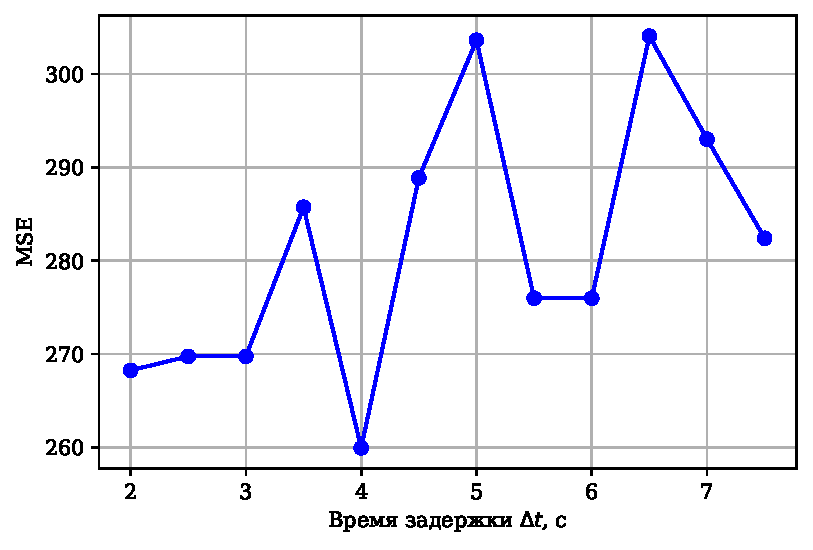
\includegraphics[scale = 0.34]{MSE_dt.pdf}
    \label{MSE_dt}
\end{figure}
\end{block}
\end{frame}
%%%%%%%%%%%%%%%%%%%%%%%%%%%%%%%%%%%%%%%%%%%%%%%%%%%%%%%%%%%%%%%%%%%%%%%%%%%%%%%%%%%%%%%%%%%%%%%%%%%%%%%%%%%%%%%%%%%%%%%%%%%%%%%%%%%%%%%%%%%%
\begin{frame}{Вычислительный эксперимент}
\begin{block}{Срез снимка фМРТ из тестовой выборки при параметрах ${\Delta t}_{opt} = 4$, $\mathrm{coef} = 4$}
\begin{figure}[h!]
    \centering
    \subfloat[Оригинальный]{\label{fig:3-orig}{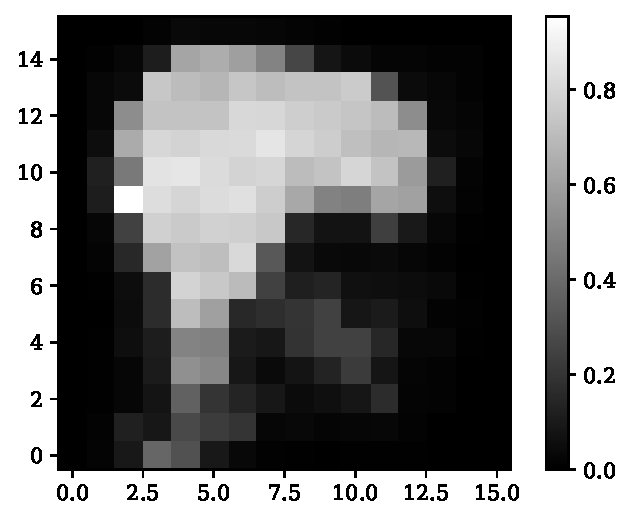
\includegraphics[width=0.3\textwidth]{sub-04-4-4-5-_-_-orig.pdf}}}
    \hfill
    \subfloat[Предсказанный]{\label{fig:3-pred}{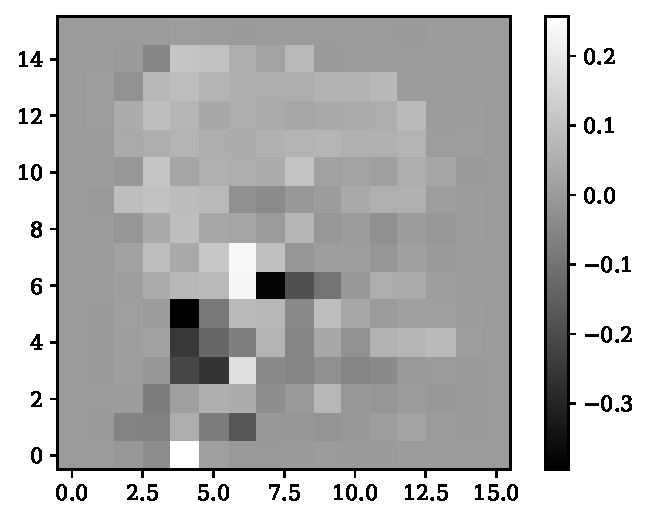
\includegraphics[width=0.3\textwidth]{sub-04-4-4-5-_-_-pred.pdf}}}
    \hfill
    \subfloat[Разность]{\label{fig:3-delta}{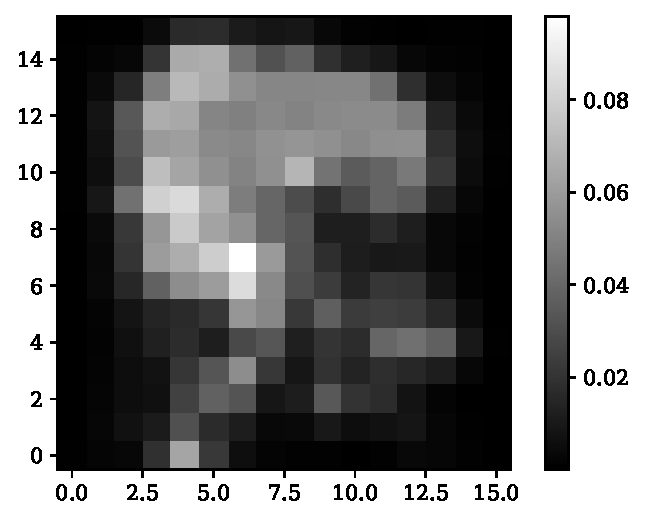
\includegraphics[width=0.3\textwidth]{sub-04-4-4-5-_-_-pred-pg.pdf}}}
  
    \label{fig:3}
\end{figure}
\end{block}


\begin{table}[h!]
		\centering
		\begin{tabular}{|c|c|c|}
			\hline
				&	MSE при обучении	&	MSE на тесте \\ \hline \hline
			MSE		& 	$253.02$	 &		$259.92$ \\ \hline
		\end{tabular}
		\caption{MSE при параметрах модели ${\Delta t}_{opt} = 4$, $\mathrm{coef} = 4$.}
		\label{table_1}
	\end{table}


\end{frame}



\begin{frame}{Вычислительный эксперимент}
\begin{block}{Варьирование гиперпараметров основной модели}
\begin{figure}[h!]
    \centering
    \subfloat[Варьирование $\Delta t$]{\label{fig_1}{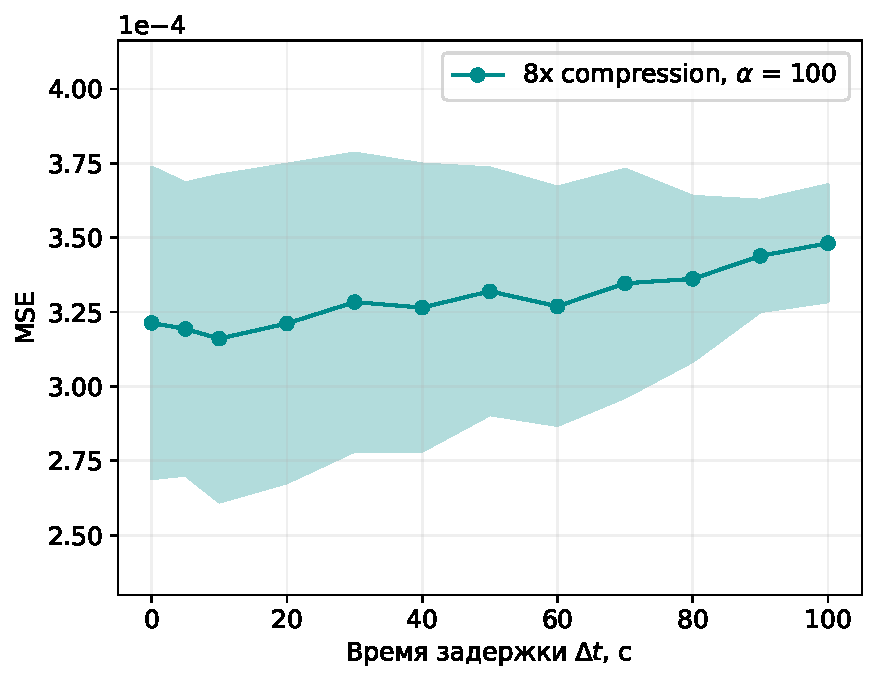
\includegraphics[width=0.46\textwidth]{subs_delta_MSE_dt.pdf}}}
    \label{subs_delta_MSE_dt}
    \hfill
    \centering
    \subfloat[Варьирование $\alpha$]{\label{fig_1}{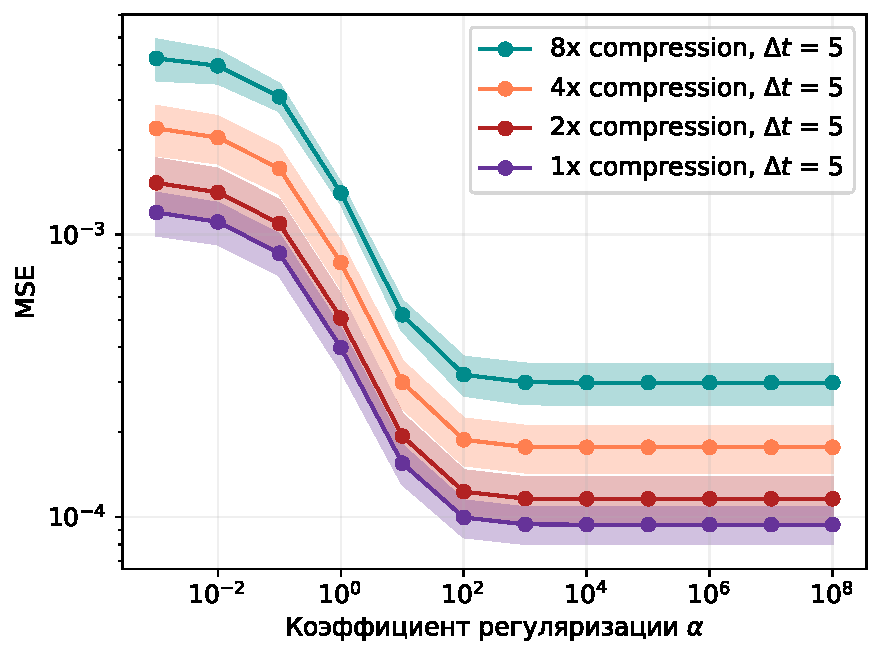
\includegraphics[width=0.46\textwidth]{subs_MSE_alpha}}}
    \label{subs_MSE_alpha}
  
\end{figure}
\end{block}

\end{frame}
%%%%%%%%%%%%%%%%%%%%%%%%%%%%%%%%%%%%%%%%%%%%%%%%%%%%%%%%%%%%%%%%%%%%%%%%%%%%%%%%%%%%%%%%%%%%%%%%%%%%%%%%%%%%%%%%%%%%%%%%%%%%%%%%%%%%%%%%%%%%%%%%%%%%%%%%%%%%%%%%%%%%%%%%%%%%%%%%%%%%%%%%%%%%%%%%%%%%%%%%%%%%%%%%%%

\begin{frame}{Анализ ошибки}
\begin{block}{Пример работы основного метода при оптимальных гиперпараметрах}
В качестве демонстрации работы алгоритма при оптимальных гиперпараметрах на рисунке ниже приведены срезы оригинального и предсказанного воксельного снимка фМРТ из тестовой выборки. 
\begin{figure}[h!]
    \centering
    \subfloat[Истинный]{\label{fig:5a}{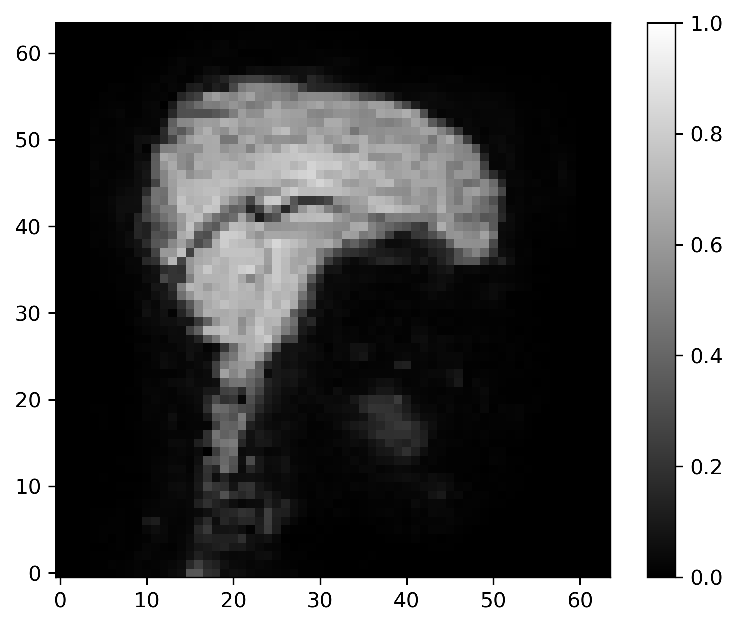
\includegraphics[width=0.33\textwidth]{sub-04-5-1-1000-100-20-_-_-test.pdf}}}
    \hfill
    \subfloat[Восстановленный]{\label{fig:5b}{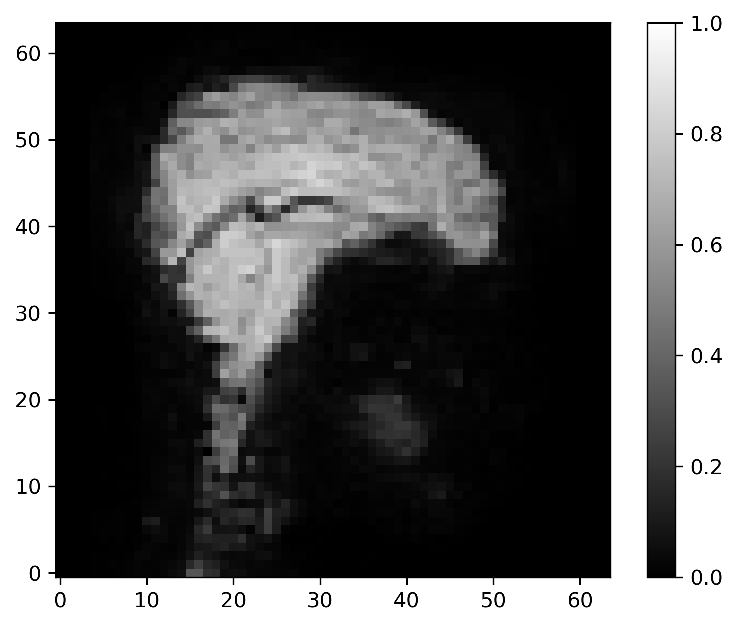
\includegraphics[width=0.33\textwidth]{sub-04-5-1-1000-100-20-_-_-predicted.pdf}}}
    \hfill
    \subfloat[Разность]{\label{fig:5c}{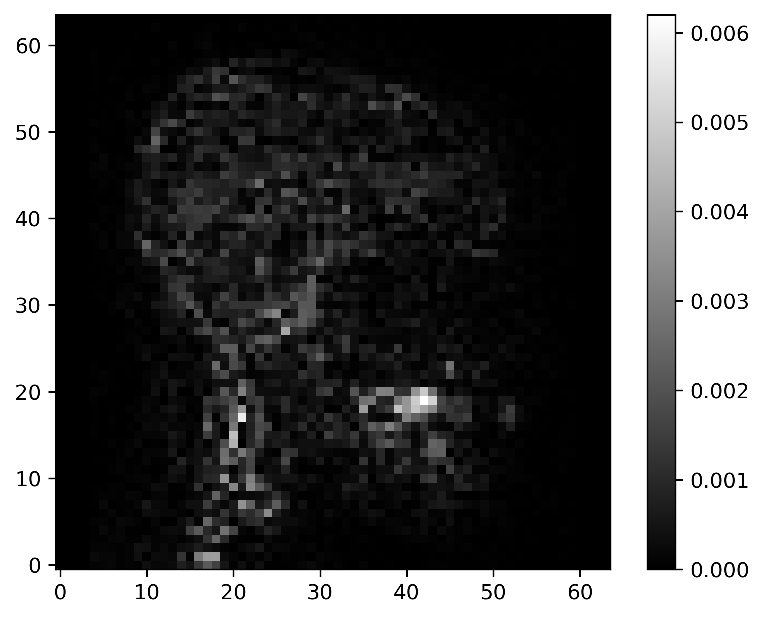
\includegraphics[width=0.33\textwidth]{sub-04-5-1-1000-100-20-_-_-difference.pdf}}}
    \label{fig:5}
\end{figure}
\end{block}

\end{frame}
%%%%%%%%%%%%%%%%%%%%%%%%%%%%%%%%%%%%%%%%%%%%%%%%%%%%%%%%%%%%%%%%%%%%%%%%%%%%%%%%%%%%%%%%%%%%%%%%%%%%%%%%%%%%%%%%%%%%%%%%%%%%%%%%%%%%%%%%%%%%%%%%%%%%%%%%%%%%%%%%%%%%%%%%%%%%%%%%%%%%%%%%%%%%%%%%%%%%%%%%%%%%%%%%%%%%
\begin{frame}{Анализ ошибки}
\begin{block}{Распределения значений компонент вектора весов основной модели.}
Для построения производилось усреднение по строкам матрицы весов $\hat{W}$, то есть усреднение по всем вокселям.
\begin{figure}[h!]
    \centering
    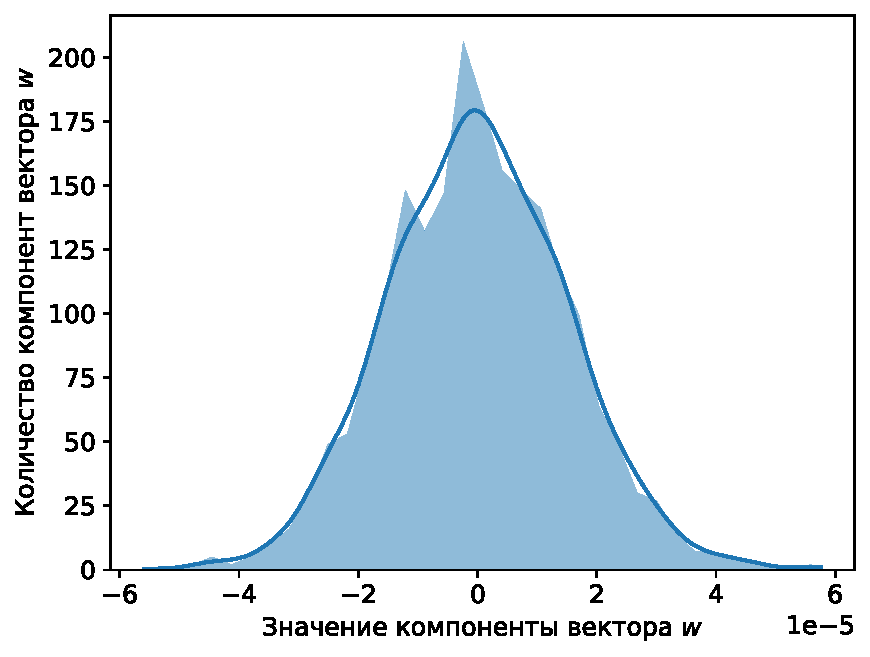
\includegraphics[width=0.46\textwidth]{mean_weight_distribution.pdf}
    \label{fig:6}
\end{figure}
График хорошо аппроксимируется плотнотью нормального распределения, что говорит о статистической значимости весов.
\end{block}

\end{frame}
%%%%%%%%%%%%%%%%%%%%%%%%%%%%%%%%%%%%%%%%%%%%%%%%%%%%%%%%%%%%%%%%%%%%%%%%%%%%%%%%%%%%%%%%%%%%%%%%%%%%%%%%%%%%%%%%%%%%%%%%%%%%%%%%%%%%%%%%%%%%%%%%%%%%%%%%%%%%%%%%%%%%%%%%%%%%%%%%%%%%%%%%%%%%%%%%%%%%%%%%%%%%%%%%%%%%
\begin{frame}{Анализ ошибки}
\begin{block}{Корректность модели: инвариантности весов модели относительно человека}
Экспериментально проверено, что модель улавливает общие для всех испытуемых зависимости между данными.
Другими словами, восстановление снимка фМРТ одного человека можно производить, используя матрицу весов другого испытуемого. Для оценки качества работы алгоритма в данном эксперименте использовалась метрика MSE на тестовой выборке.
Результаты представлены в таблице ниже:

	\begin{table}[h!]
		\centering
		\begin{tabular}{|c|c|c|}
			\hline
			Матрица весов	&	Истинная	&	Подмешанная \\ \hline \hline
			MSE		& 	$1.02 \cdot 10^{-4}$	 &		$1.05 \cdot 10^{-4}$ \\ \hline
		\end{tabular}
		\label{table_2}
	\end{table}
\end{block}

\end{frame}
%%%%%%%%%%%%%%%%%%%%%%%%%%%%%%%%%%%%%%%%%%%%%%%%%%%%%%%%%%%%%%%%%%%%%%%%%%%%%%%%%%%%%%%%%%%%%%%%%%%%%%%%%%%%%%%%%%%%%%%%%%%%%%%%%%%%%%%%%%%%%%%%%%%%%%%%%%%%%%%%%%%%%%%%%%%%%%%%%%%%%%%%%%%%%%%%%%%%%%%%%%%%%%%%%%%%
\begin{frame}{Анализ ошибки}
\begin{block}{Корректность модели: результаты работы модели на случайном шуме}
Первоначально модель обучена на оригинальных изображениях из видеоряда. По шумовым данным и матрице весов $\hat{W}$ получена последовательность изменений между соседними снимками фМРТ. Результат предсказания последнего снимка по первому приведен ниже:
\begin{figure}[h!]
    \centering
    \subfloat[Истинный]{\label{fig:8a}{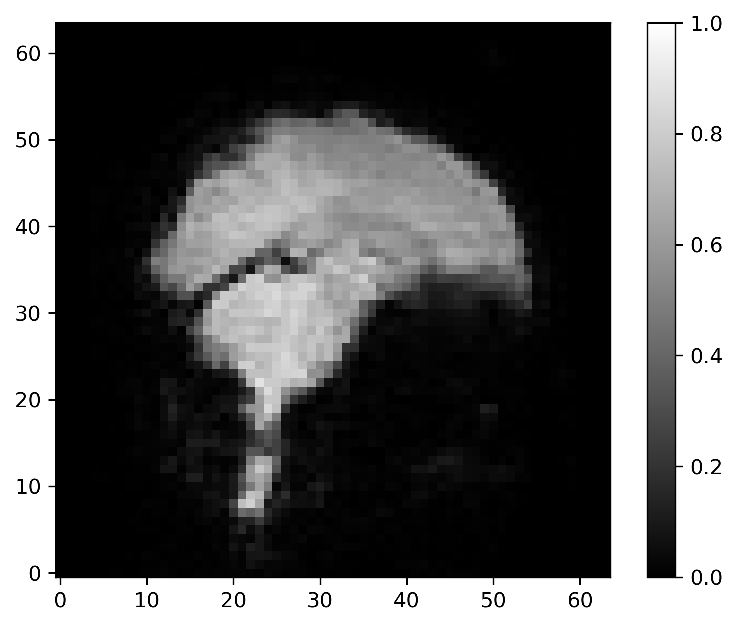
\includegraphics[width=0.33\textwidth]{sub-35-5-1-1000--1-20-_-_-recovered-test_noised.pdf}}}
    \hfill
    \subfloat[Восстановленный по шуму]{\label{fig:8b}{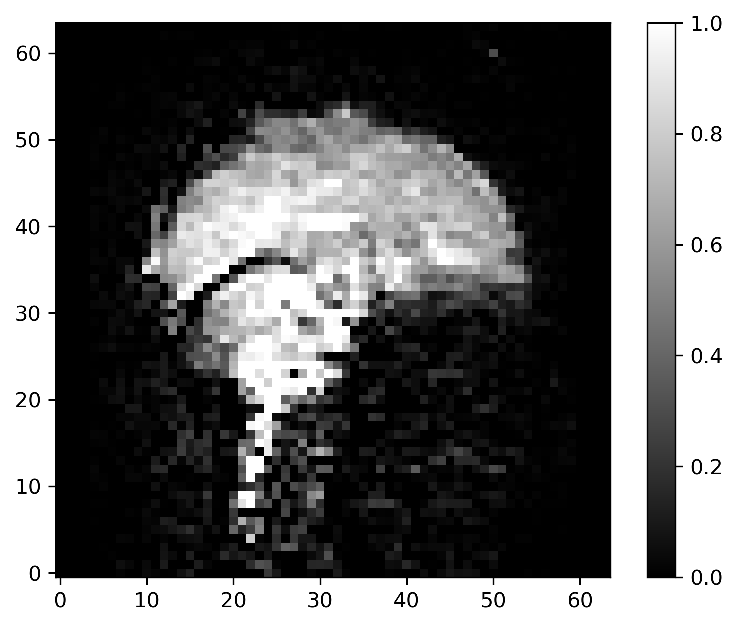
\includegraphics[width=0.33\textwidth]{sub-35-5-1-1000--1-20-_-_-recovered-predicted_noised.pdf}}}
    \hfill
    \subfloat[Разность]{\label{fig:8c}{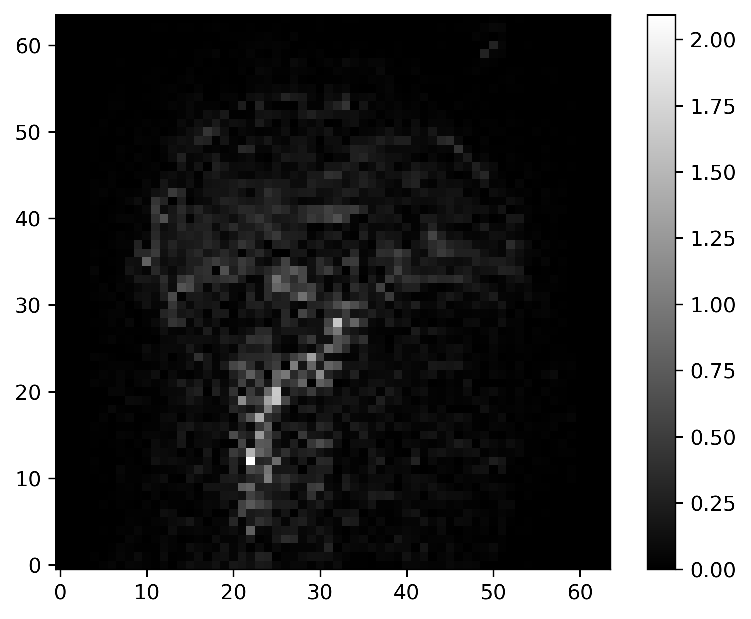
\includegraphics[width=0.33\textwidth]{sub-35-5-1-1000--1-20-_-_-recovered-difference_noised.pdf}}}
    \label{fig:8}
\end{figure}
\end{block}
\end{frame}
%%%%%%%%%%%%%%%%%%%%%%%%%%%%%%%%%%%%%%%%%%%%%%%%%%%%%%%%%%%%%%%%%%%%%%%%%%%%%%%%%%%%%%%%%%%%%%%%%%%%%%%%%%%%%%%%%%%%%%%%%%%%%%%%%%%%%%%%%%%%%%%%%%%%%%%%%%%%%%%%%%%%%%%%%%%%%%%%%%%%%%%%%%%%%%%%%%%%%%%%%%%%%%%%%%%%
\begin{frame}{Анализ ошибки}
\begin{block}{Корректность модели: результаты работы модели на случайном шуме}
В таблице приведены среднеквадратичные ошибки.
Ошибка на шуме на порядок больше, что подтверждает наличие корреляции между показаниями датчиков и изображениями из видеоряда.
\begin{table}[h!]
    \centering
    \begin{tabular}{|c|c|c|}
        \hline
        Выборка	&	Истинная	&	Случайный шум \\ \hline \hline
        MSE		& 	$2 \cdot 10^{-3}$	 &		$10^{-1}$ \\ \hline
    \end{tabular}
    \label{table_3}
\end{table}
\end{block}
\end{frame}
%%%%%%%%%%%%%%%%%%%%%%%%%%%%%%%%%%%%%%%%%%%%%%%%%%%%%%%%%%%%%%%%%%%%%%%%%%%%%%%%%%%%%%%%%%%%%%%%%%%%%%%%%%%%%%%%%%%%%%%%%%%%%%%%%%%%%%%%%%%%%%%%%%%%%%%%%%%%%%%%%%%%%%%%%%%%%%%%%%%%%%%%%%%%%%%%%%%%%%%%%%%%%%%%%%%%
\begin{frame}{Выводы}
\begin{itemize}
    \item В работе построен базовый и основной метод аппроксимации показаний датичков фМРТ по видеоряду, просматриваемому человеком. 
    \item Результаты экспериментов подтверждают наличие корреляции между данными.
    \item Приведенные графики подтверждают предположение о наличии задержки между моментом получения информации зрительными органами и реакцией мозга на эту информацию.
    \item Качество работы основного метода в разы превосходит качество работы базового алгоритма. 
    Особенность основного метода заключается в учете временной зависимости между снимками за счет предсказания разности между соседними показаниями датчиков фМРТ. 
\end{itemize}
\end{frame}
\end{document}